\documentclass[xcolor=dvipsnames]{beamer}

\title{Improving the Interoperability of Java and Clojure}
\author{Stephen Adams}
\institute{University of Minnesota: Morris}
\date{April 14th, 2012}

% Setup appearance:
\usepackage{beamerthemesplit}
\usecolortheme[named=Brown]{structure} 
%\usetheme{Darmstadt}
%\usefonttheme[onlylarge]{structurebold}
%\setbeamerfont*{frametitle}{size=\normalsize,series=\bfseries}
%\setbeamertemplate{navigation symbols}{}


% Standard packages

\usepackage[english]{babel}
\usepackage[latin1]{inputenc}
\usepackage{times}
\usepackage[T1]{fontenc}
\usepackage[round]{natbib}


% Setup TikZ

\usepackage{tikz}
\usetikzlibrary{arrows}
\tikzstyle{block}=[draw opacity=0.7,line width=1.4cm]

\begin{document}

\begin{frame}
	\titlepage
\end{frame}

\section*{Outline}
	\section{Introduction}
	
	\begin{frame}{A little reminder about Java}
		An object-oriented language released by Sun Microsystems in 1995.
		\begin{itemize}
		\item Compiled to Java bytecode
		\item Java bytecode is run on the Java Virtual Machine
		\item Second language in TIOBE programming Community Index (as of April 2012)
		\end{itemize}
	\end{frame}
		
	\begin{frame}
		The Clojure programming language was released in 2007 by the software developer Rich Hickey. Clojure was designed with four features in mind:
		\pause
		\begin{block}{The Four Features of Clojure}
		\begin{itemize}
			\item A Lisp
			\item Functional programming
			\item Symbiosis with an established platform
			\item Designed for concurrency
		\end{itemize}
		\end{block}
	\end{frame}
	
	\begin{frame}{LISP and Functional Programming}
		\begin{itemize}
		\item Lisp was developed in 1958
		\item The earliest functional language
		\item Emphasizes the application of functions
		\item Imperative programming emphasizes changes in state
		\end{itemize}
	\end{frame}
	
	\begin{frame}{Functional Programming and concurrency}
		\begin{itemize}
		\item Functional languages have immutable data
		\item No state = no side effects
		\item A function will always return the same results given the same arguments
		\item Easier to predict behavior of a program in a concurrent environment
		\end{itemize}
	\end{frame}
	
	\begin{frame}{Who Clojure is for?}
			\begin{itemize}
				\item Need to parallelize your work?
				\item Are you tired of Java?
		\pause
				\item Have a project already written in Java?
				\item Have a Java library you use a lot?
			\end{itemize}
	\end{frame}
	
	\begin{frame}{Who this talk is for}
	"Clojure does Java better than Java" - Stuart Halloway, at the Greater Atlanta Software Symposium, 2009.
	\end{frame}
		
	\begin{frame}
		\tableofcontents
	\end{frame}
	
	\section{Introduction to Clojure}
		\subsubsection{Basic Clojure syntax}
		\begin{frame}[fragile]
		\frametitle{Prefix Notation}
		\begin{verbatim}
			(+ 2 3)
			=> 5
		\end{verbatim}
		\pause
		\begin{verbatim}
		(+ 2 3 4)
		=> 9
		(inc 4)
		=> 5
		\end{verbatim}
		\end{frame}
		
		\begin{frame}[fragile]
		\frametitle{Clojure Data Structures}
			\begin{itemize}			
			\item Many of Clojure's data structures are just Java data structures; strings, characters, and all numbers are just Java types.
			\pause
			\item Clojure provides its own collections.
			\end{itemize}
		\end{frame}
		\begin{frame}
		Every Clojure collection is denoted by a different literal symbol pair.
			\begin{block}{Collection Literals}
				\begin{table}[H]
				\begin{tabular}{ | l | c | }
				\hline
				List & (1 2 3 4) \\ \hline
				Vector & ["apple" "banana" "orange"] \\ \hline
				Hashmap & \{ :name "Stephen Adams" :phone 555555555 \} \\ \hline
				\end{tabular}
				\end{table}
			\end{block}
		\end{frame}
		
		\begin{frame}[fragile]
		\frametitle{Keywords}
		\begin{itemize}
			\item Symbolic identifiers, denoted with a leading colon
			\item The colon is not considered part of the keyword
			\item Keywords evaluate to themselves
			\item Very fast equality tests 
		\end{itemize}
		\begin{verbatim}
		:keyword
		=> :keyword
		\end{verbatim}
		\end{frame}
		
		\begin{frame}[fragile]
		\frametitle{Variables and Functions}
		\begin{verbatim}
		(def vect [1 2 3 4 5])
		
		(defn square [x] 
		   (* x x))
		\end{verbatim}	
		\end{frame}
		
%		\begin{frame}[fragile]
%		\frametitle{Namespaces}
%			\begin{verbatim}
%				(ns some.SampleNamespace
%				   (:import javax.swing.JFrame))
%			\end{verbatim}
%			\begin{itemize}
%				\item Provide a symbolic identifier for pieces of Clojure code
%			\end{itemize}
%		\end{frame}
		
		
%		\begin{frame}[fragile]
%		\frametitle{Macros}
%			Textual transformations that happen before evaluation. \newline
%			Macro expands one piece of code to another.
%			\begin{block}{Unless Macro}
%				\begin{verbatim}
%					(ns macro.Example)
%
%					(defmacro unless [conditional caseA caseB]
%					   `(if (not ~conditional) ~caseA ~caseB))
%					
%   					(unless false (println "Will print") 
%   					   (println "Will not print"))
%
%					(if (not false) (println "Will print") 
%					   (println "Will not print"))
%				\end{verbatim}
%			\end{block}
%		\end{frame}
	\section{Functional Programming in Clojure}
		\begin{frame}{The functional features of Clojure}
			Functional programming primarily refers to two language features:
			\begin{itemize}
			\item First class functions
			\item Anonymous functions
			\end{itemize}		
			Clojure supports both of these features.
		\end{frame}
		\subsubsection{First Class Functions in Clojure}
		\begin{frame}[fragile]
		\frametitle{First Class Functions}
		\framesubtitle{Passing functions to other functions}
		
		\begin{verbatim}
		(defn square [x] 
		   (* x x))
		\end{verbatim}
		\pause
		\begin{verbatim}
		(map square [1 2 3 4 5])
		=> [1 4 9 16 25]
		\end{verbatim}
		\pause
		\begin{verbatim}
		(reduce + [1 2 3 4 5])
		=> 15
		\end{verbatim}
		\end{frame}
		\subsubsection{Anonymous Functions in Clojure}
		\begin{frame}[fragile]
		\frametitle{Anonymous Functions}
		\begin{verbatim}
			(defn all-same? [vect]
			 (if (empty? vect) 
			  true
			  (every? 
			   (fn [x] (= (first vect) x )) (rest vect))
		\end{verbatim}		
		\end{frame}
	\section{Java Interop}
		\begin{frame}{Introduction to Java Interop}
			The idea for Clojure always involved interoperability with an existing language. Java was chosen for various reasons:
			\begin{itemize}
				\item Access to previously written Java libraries
				\item Already implemented, garbage collection and other memory \& resource management tools.
				\item JVM is OS agnostic.
			\end{itemize}
		\end{frame}
		\subsection{Basic Java calling}
		
		\begin{frame}[fragile]
		\frametitle{The dot special form}
			\begin{itemize}
				\item Provides basic access to Java fields and methods
				\item Can also be read as ``in the scope of."
			\end{itemize}
			\begin{verbatim}
			(. "fred" toUpperCase)
			=> "FRED"
			\end{verbatim}
			\pause
			\begin{verbatim}
			"fred".toUpperCase();
			\end{verbatim}
		\end{frame}
		
		\begin{frame}[fragile]
		\frametitle{The dot special form cont.}
		\begin{verbatim}
		(.toUpperCase "fred")
		\end{verbatim}		
		\pause
		Accessing Static methods and fields
		\begin{verbatim}
		(. Math PI)
		=> 3.141592653589793
		\end{verbatim}		
		\begin{verbatim}
		(Math/PI)
		=> 3.141592653589793
		(Math/abs -2)
		=> 2
		\end{verbatim}		
		\end{frame}
		
		\subsection{Java Objects in Clojure}
		\begin{frame}[fragile]
		\frametitle{Object Construction and modification}
		\begin{verbatim}
	    (new StringBuffer "fred")
	    => #<StringBuffer fred>
		\end{verbatim}
		\pause
		\begin{verbatim}
		    (doto (new StringBuffer "fred") 
	    (.setCharAt 0 \F) 
	    (.append " is a nice guy!"))
	    => #<StringBuffer Fred is a nice guy!>
	    \end{verbatim}	
		\end{frame}
		
		\begin{frame}[fragile]
		\frametitle{Object Construction and modification cont.}
		\begin{verbatim}		
		public class ExampleBuffer {
		   public static void main(String[] args){
		      StringBuffer buff = new StringBuffer("fred");
		      buff.setCharAt(0, "F");
		      buff.append(" is a nice guy");
		   }
		}
		\end{verbatim}
		\end{frame}
		
		\subsection{Custom types in Clojure}
		\begin{frame}{Many ways of defining a type}
		\tiny By Chas Emerick, from: http://bit.ly/IiozRP		
		\begin{center}
			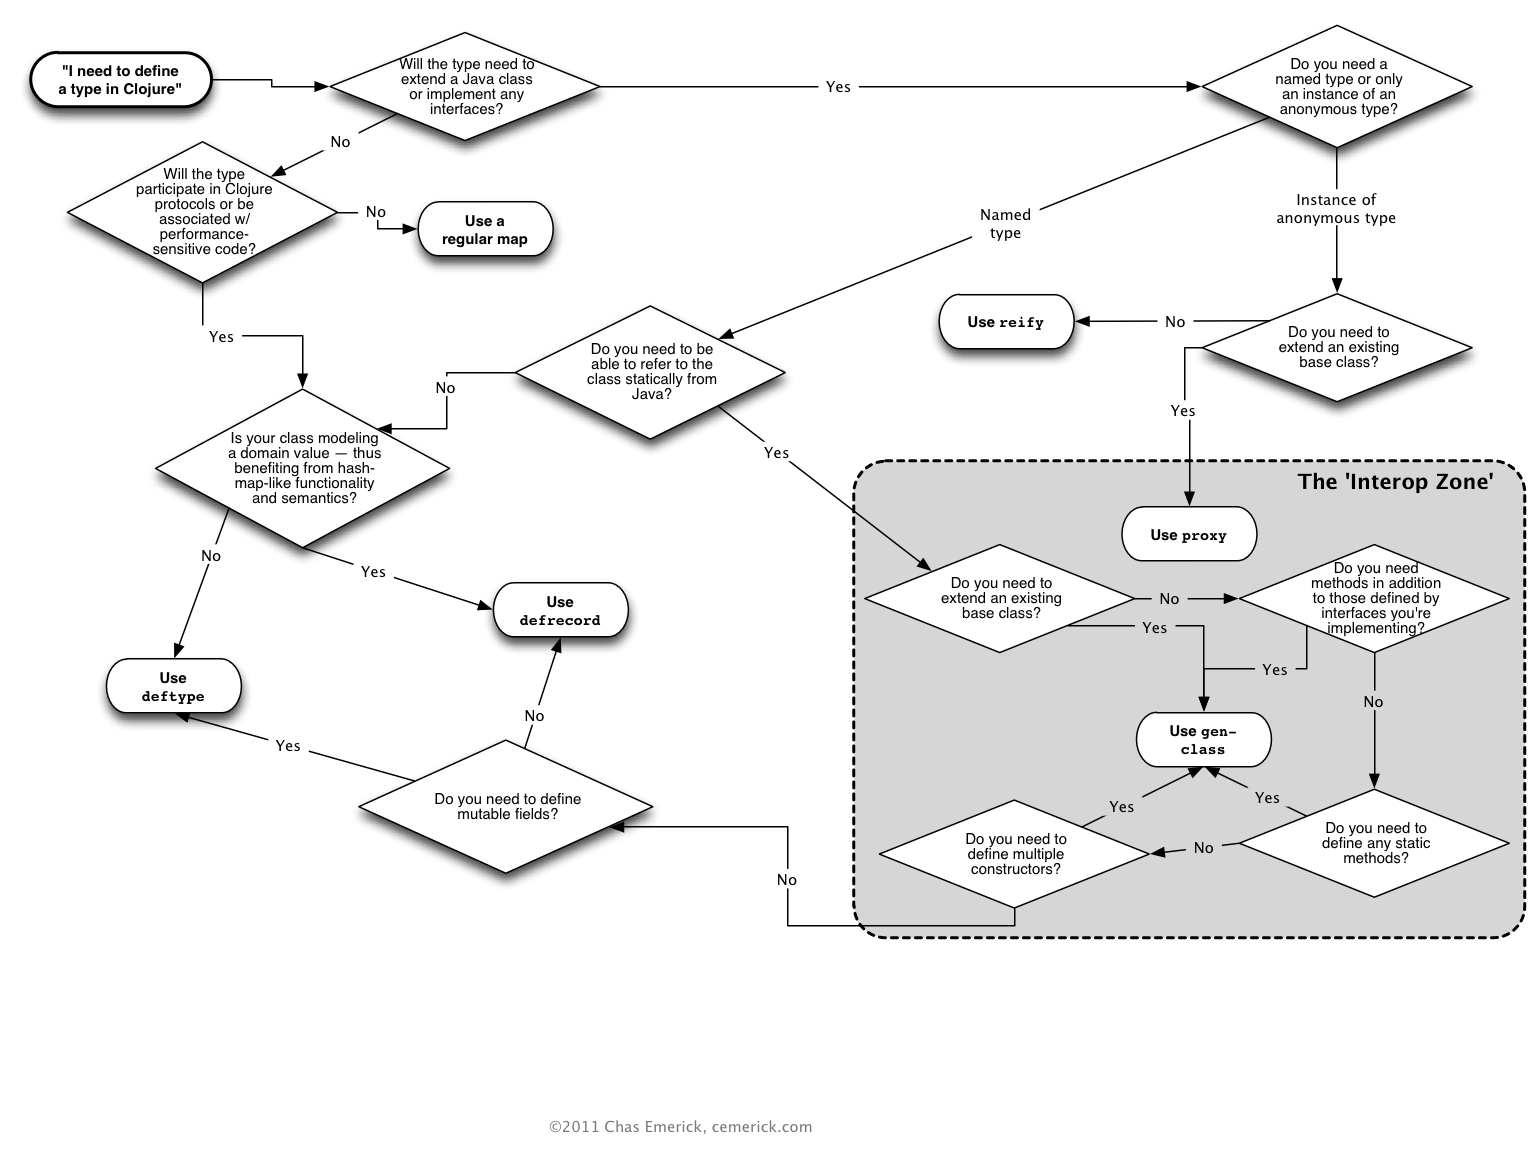
\includegraphics[scale=.2]{choosingtypeforms.png}
		\end{center}
		\end{frame}
		
		\begin{frame}{Many ways of defining a type}
		\begin{center}
			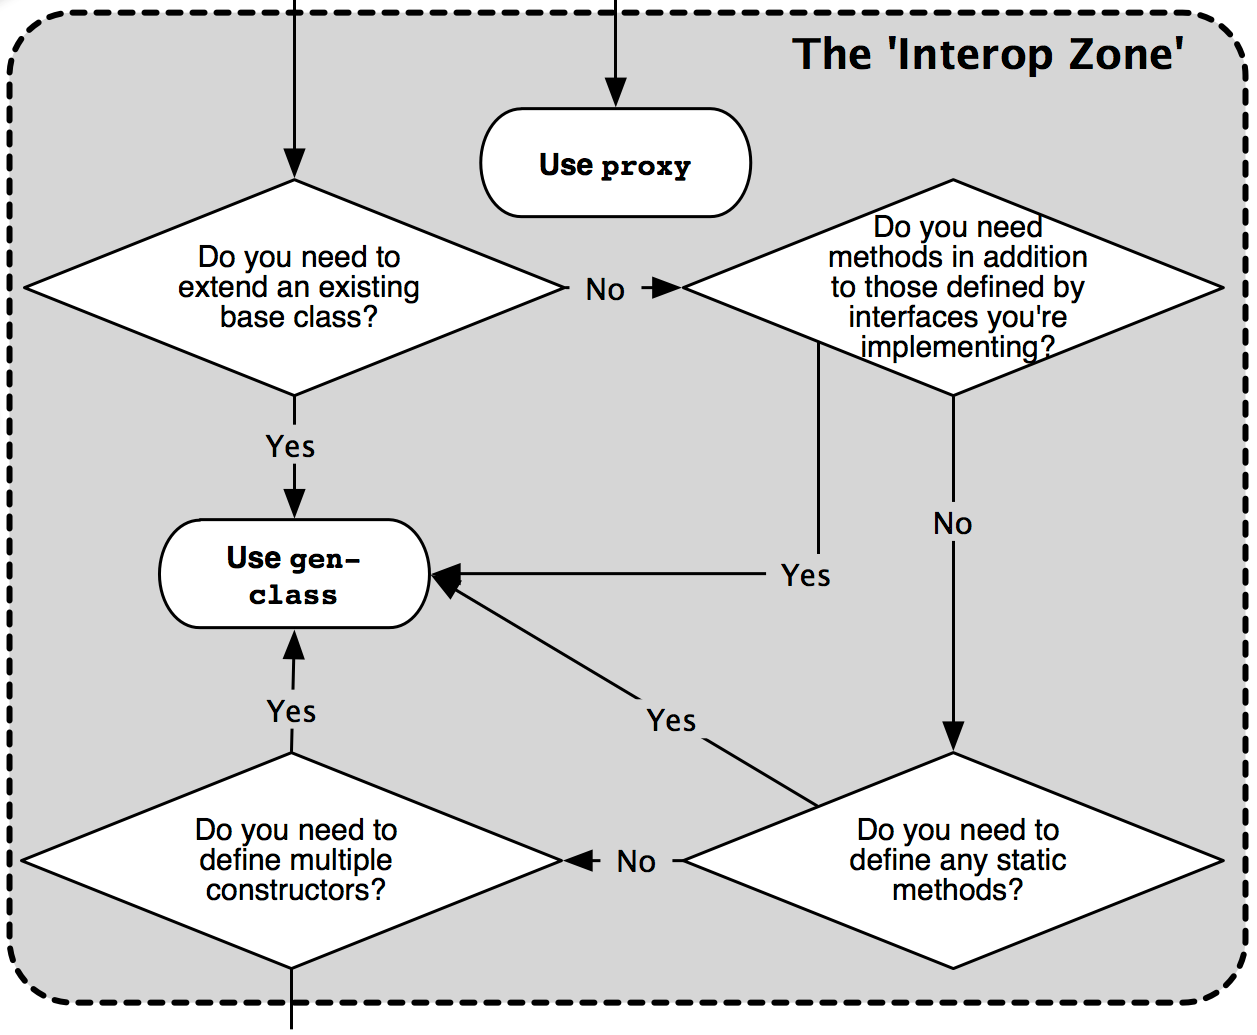
\includegraphics[scale=.15]{choosingtypeformszoom.png}
		\end{center}
		\end{frame}
		
		\begin{frame}{The Java interop zone}
			Clojure functions designed to work with existing Java code.
			\begin{block}{The interop zone}
			\begin{itemize}			
			\item proxy
			\item gen-class
			\end{itemize}
			\end{block}
		\end{frame}

	
	\begin{frame}{Proxy}
	\begin{itemize}
	\item Must implement a Java interface or extend a Java class
	\item Creates a single instance of an anonymous Java class
	\item Cannot define methods not declared by a superclass or interface
	\end{itemize}
	\end{frame}	

	%\begin{frame}[fragile]
	%\frametitle{Proxy cont.}
	%\begin{verbatim}
	%public interface TestInterface {
	%	int square(int x);
	%}
	%\end{verbatim}
	%\pause
	%\begin{verbatim}
	%(def test-inter 
	%  (proxy [TestInterface] [] (square [x] (* x x))))
	%\end{verbatim}
	%\pause
	%\begin{verbatim}
	%(. test-inter square 5)
	%=> 25
	%\end{verbatim}
	%\end{frame}
	
	\begin{frame}[fragile]
	\frametitle{Proxy cont.}
	\begin{verbatim}
	(defn add-mousepressed-listener
     [component func args]
      (let [listener (proxy [MouseAdapter] []
                     (mousePressed [event]
                        (apply func event args)))]
      (.addMouseListener component listener)
    listener))
	\end{verbatim}
	\end{frame}
	
	\begin{frame}{Gen-class}
	\begin{itemize}	
	\item Proxy will only allow you to do so much because you can only overload functions defined by a super class or interface.
	\pause
	\item There are cases when defining your own Java methods and objects is necessary.
	\item For instance working with a library that requires you to extend some object. 
	\end{itemize}
	\end{frame}
	
	\begin{frame}[fragile]
	\frametitle{Gen-class cont.}
		\begin{verbatim}
	  (gen-class 
	      :prefix "method-"))
	  
	(defn method-toString
	  [this]
	  "Hello, world!")
	  
	\end{verbatim}
	\pause
	\begin{verbatim}
	(def aClass (new some.Example))
	(.toString aClass)
	=> "Hello, world!"
	\end{verbatim}
	\end{frame}
	
	\begin{frame}[fragile]
		\begin{verbatim}
	(gen-class
	  :name  some.Example.classA
	  :prefix classA- )
	  
	(gen-class
	  :name some.Example.classB
	  :prefix classB- )
	  
	(defn classA-toString
	  [this]
	  "I'm an A.")
	  
	(defn classB-toString
	  [this]
	  "I'm an B.")
	\end{verbatim}
	\end{frame}
	
	\section{Conclusion \& References}
	\begin{frame}{Java - Clojure Relationship}
	"Clojure does Java better than Java" - Stuart Halloway, at the Greater Atlanta Software Symposium, 2009.
	\linebreak
	Proxy is an example of this.
	\end{frame}
	
	\begin{frame}{Java - Clojure Relationship}
	\begin{itemize}	
	\item You want to program Clojure in Clojure, not Java.
	\item Gen-class and, to some extent, proxy break from Clojure-like syntax.
	\item These functions should be used sparingly.
	\item C. Emerick's figure (http://bit.ly/IiozRP).
	\end{itemize}
	\end{frame}
	
	\begin{frame}{Recommendations}
	\begin{itemize}
		\item Push Clojure's native abstractions into interop zone, possibly macros.
		\item Centralize documentation sources.
		\item Streamline IDE setup for beginners.
	\end{itemize}
	\end{frame}
	
	\begin{frame}{Why this matters}
		``The killer app for Clojure is the JVM itself. Everyone's fed up with the Java language, but understandably we don't want to abandon our investment in the Java Virtual Machine and its capabilities: the libraries, the configuration, the monitoring, and all the other entirely valid reasons we still use it."  
		\newline
		Steve Yegge, in the foreward to Joy of Clojure.
	\end{frame}
	
	\begin{frame}{References}
	\begin{itemize}
	\item CLOJUREDOCS.ORG. Mar. 2012. [Online; accessed March-2012].
	\item CLOJURE.ORG. Mar. 2012. [Online; accessed March-2012].
	\item Fogus, M., and Houser, C. The Joy of Clojure, Manning Publications.
	\item Halloway, S. Clojure-Java interop: A better Java than Java. QCon.
	\end{itemize}
	\end{frame}
\end{document}
